\section{Classification}
For any class we estimate the probability of being in such class:

    $\pi_j(x) = \mathbb{P}(Y = j\mid X=x)$

The \textbf{Bayes estimator} is $\mathcal{C}(x) = \arg\max_j\pi_j(x)$.\\
\textbf{KNN:} here we take the $K$ nearest neighbours and we have them vote, $K$ big = bias, $K$ small = variance.
\begin{codebox}{r}{KNN}
library(FNN)
pred.knn <- knn.reg(train = matrix(dtrain[,1],ncol=1), test=matrix(dtest[,1], ncol=1), y = ytrain, k=i)
  results.knn[i] <- mean((ytest - pred.knn$pred)^2
fit <- glm(y ~ x, family = binomial, data = heart)
\end{codebox}
\textbf{Linear \& quadratic discriminant analysis:} 
Here we assume $X\mid Y = j \sim \mathcal{N}(\mu_j,\Sigma)$. To approximate we 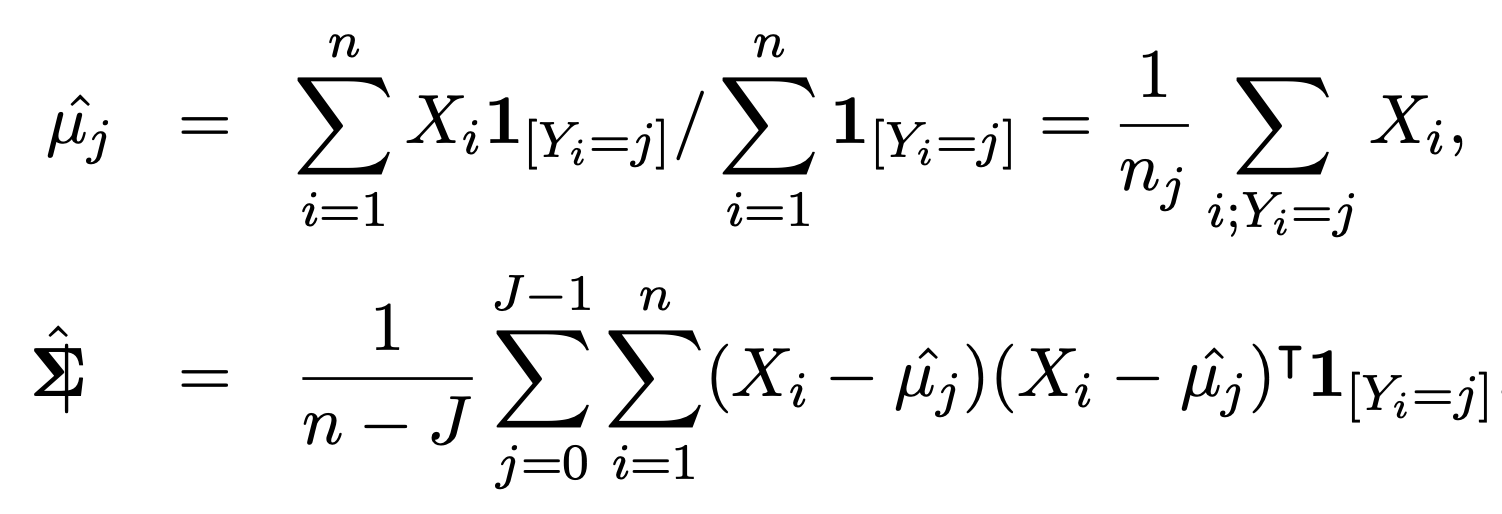
\includegraphics[width = 5cm]{LDA.png}\\

\textbf{Quadratic discriminant analysis:} Here we can do group-wise $\Sigma$ by only looking at elements in the group and by correcting with $\frac{1}{n_j-1}$ instead of $\frac{1}{n-j}$.
\begin{codebox}{r}{Linear \& Quadratic Discriminant analysis}
library(MASS)
c_lda<-lda(x=data[,c("x1","x2")],grouping=data[,"y"])
c_qda<-qda(x=data[,c("x1","x2")],grouping=data[,"y"])
# Pred. performance assessment, adjust FP, FN penalty
\end{codebox}
\textbf{Logistic regression:} Let $\pi(x) = \mathbb{P}(Y=1\mid X = x)$. We estimate with a linear model $g(x) = \text{logit}(\pi(x)) = \log\frac{\pi(x)}{1-\pi(x)}$. Assuming $g(x) = X\beta$ and we look at the log-likelyhood we get:
$\ell(\beta;Y,X)=\sum_{i=1}^n\left(Y_i \beta^Tx_i - \log\left(e^{\beta^Tx_i} +1\right)\right)$\\
Minimizing this is not trivial and we use gradient descent\\
\begin{codebox}{r}{Logistic regression}
mod <- glm(y ~ ., data = data, family = "binomial")
#family="binomial" is what makes a logistic reg.
predict(mod, type = "response") # return the probability of being 1
# for multinomial regression
class_multinom <- multinom(y ~ . , data = data)
\end{codebox}
\textbf{More classes techniques:}\\
1) (one versus rest). You train a model per class with that class against the rest and we get $\pi_j(x)$ (but they don't add up to one, hence we normalize). $g(x) = \log(\pi_j(x)/\pi_0(x))$\\
2) One can use multinomial dist. which generalizes Bernoulli\\
3) We train $J-1$ with the classes against a reference class $J=0$\\
4) We train a model to distinguish each class from each other. In total $\binom{J}{2}$ models\\
5) In the case when classes are ordered: $\text{logit}(\mathbb{P}(Y\leq k \mid x))=\alpha_k +g(x)$ with $\alpha_0\leq\alpha_1\leq\dots\leq \alpha_{J-1}$\\
\textbf{Confusion Matrix}\\ % Maybe some color coding would be nice here

\begin{tabular}{|l|l|l|}
\hline
\begin{tabular}[c]{@{}l@{}}Total pop.\\ TP=P+N\end{tabular}        & \begin{tabular}[c]{@{}l@{}}Predicted\\ Positive PP\end{tabular}                & \begin{tabular}[c]{@{}l@{}}Predicted\\ Negative PN\end{tabular}                \\ \hline
Positive P                                                         & TP                                                                             & FN                                                                             \\ \hline
Negative N                                                         & FP                                                                             & TN                                                                             \\ \hline
\begin{tabular}[c]{@{}l@{}}Prevalence\\ P/(P+N)\end{tabular}       & \begin{tabular}[c]{@{}l@{}}Precision PPV\\ TP/PP=1-FDR\end{tabular}            & \begin{tabular}[c]{@{}l@{}}False Omission Rate\\ FOR=FN/PN=1-NPV\end{tabular}  \\ \hline
\begin{tabular}[c]{@{}l@{}}Accuracy\\ (TP+TN)/(P+N)\end{tabular}   & \begin{tabular}[c]{@{}l@{}}False Discov. Rate\\ FDR=FP/PP=1-PPV\end{tabular}   & \begin{tabular}[c]{@{}l@{}}Neg. Predictive Val.\\ NPV=TN/PN=1-FOR\end{tabular} \\ \hline
\begin{tabular}[c]{@{}l@{}}Balanced Acc\\ (TPR/TNR)/2\end{tabular} & \begin{tabular}[c]{@{}l@{}}F\_1 Score=\\ (2xPPVxTPR)\\ /(PPV+TPR)\end{tabular} &                                                                                \\ \hline
\end{tabular}
TPR (sensitivity) = TP/P $\qquad\qquad\qquad\quad$  TNR (specitivity) = TN/N\\
FPR (1-specitivity) = 1-TNR = FP/N  \qquad \hbox{     } FNR = 1-TPR = FN/P\\
\textbf{ROC (Receiver Operating Characteristic):}
We predict $\hat Y(x) = \mathbb{I}(\pi(x)\geq p_0)$. Changing all values of $p_0 \in [0, 1]$, we look at TPR vs FPR. \\
\begin{codebox}{r}{Evaluation}
#l is a vector of 0/1 (the truth)
#p is a vector of predicted probs to be 1
pred <- prediction(predictions = p, labels = l)
perf <- performance( pred, "tpr", "fpr" )
plot(perf)# plots the ROC curve
perf.c <- performance(pred, "cost", cost.fp = 1, cost.fn = 2)
plot(perf.cost)
#plots the cost changing the cutoff (cost.fp and cost.fn can be setted to have an asym loss)
#to add cross-validation
all.y.true <- all.y.pred <- vector("list", length=K)
#and we fill them with CV, then to make average ROC:
pred.cv <- prediction(all.y.pred, all.y.true)
perf.cv <- performance(pred.cv, "tpr", "fpr" )
plot(perf.cv, avg = "threshold")
plot(perf, col = 2, add = TRUE)
\end{codebox}
%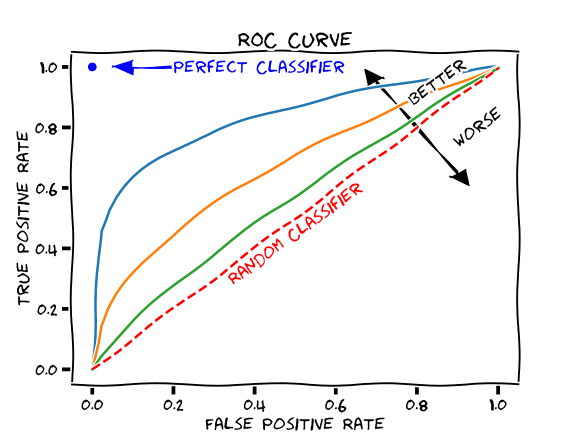
\includegraphics[width = 5cm]{ROC.png}\\